\documentclass[11pt,a4paper]{article}

\usepackage[a4paper]{geometry}
\usepackage{fullpage}
\usepackage{fancyhdr}
\usepackage{lastpage}
\usepackage{mathtools}
\usepackage{gensymb}
\usepackage{listings}
\usepackage{fontspec}
\usepackage{color}
\usepackage{graphicx}
\usepackage{wrapfig}
\usepackage{tabularx}
\usepackage{hyperref}
\usepackage[french]{babel}
\usepackage{indentfirst}
\usepackage{multicol}
%\usepackage{float}
\usepackage{mdwlist}

\newcommand\vartitle{Implémentation du protocole TFTP}
\newcommand\varauthor{Kevin Estalella, Federico Lerda, Federico Pfeiffer}
\newcommand\vardate{\today}

\title{\vartitle}
\author{\varauthor}
\date{\vardate}

\pagestyle{fancyplain}
\lhead[\vartitle]{\vartitle}
\chead[]{}
\rhead[\varauthor]{\varauthor}
\lfoot[]{}
\cfoot[\thepage\ of \pageref{LastPage}]{\thepage\ of \pageref{LastPage}}
\rfoot[]{}

\renewcommand{\headrulewidth}{0.2mm}
\renewcommand{\footrulewidth}{0mm}

\setlength{\headsep}{40pt}

\setlength{\columnsep}{30pt}

\setlength{\parindent}{0mm}
\setlength{\parskip}{2mm}

\setcounter{secnumdepth}{3}
\setcounter{tocdepth}{2}


\hypersetup{
  hidelinks,
  pdfstartview={FitV},
  pdftitle={\vartitle},
  pdfauthor={\varauthor}
}

\begin{document}

  \begin{titlepage}
    \maketitle

    \thispagestyle{empty}

    \begin{abstract}
    \begin{center}
    Ce rapport décrit l'implémentation du protocole TFTP dans le langage python. 
    \end{center}
    \end{abstract}

    \vspace{1cm}

    \tableofcontents

  \end{titlepage}


  \newpage


  \section{Présentation}

  \par Le projet consiste en l’implémentation du protocole TFTP. Ce protocole est une version light du protocole FTP. Le but de ce projet est d’implémenter une version simplifiée de TFTP en utilisant les méthodes vues en cours. Le protocole est implémenté en se basant sur la RFC 1350.

  \section{Protocole TFTP}
  
  \subsection{Vue d'ensemble}
  
  \par Le protocole TFTP est un protocole servant à envoyer / recevoir des fichiers entre un client et un serveur. Les deux parties peuvent se comporter comme émetteur et récepteur. La transmission d'un fichier débute par une requête de la part du client, dans le but de demander à envoyer un fichier (requête représentée par un paquet WRQ), ou dans le but de demander à recevoir un fichier (requête représentée par un paquet RRQ). Si le serveur accepte, le transfert de fichier commence. 
  
  \par Les fichiers sont transmis par paquets de données d'une taille de 512 Octets. Un paquet de données contenant moins de 512 Octets signifie qu'il s'agit le dernier paquet.
  
  \par Chaque paquet contient un numéro de paquet et est acquitté par le destinataire par un paquet ACK; l'émetteur d'un paquet de données doit attendre la réception d'un ACK avant d'envoyer le paquet de données suivant.  En cas d'erreur, un paquet ERR est envoyé et le transfert est annulé et terminé. 
  
  \subsection{Machines d'états}

  \par Les machines d'états suivantes ont été créés en se basant sur le descriptif de la RFC 1350. 
  
  \subsubsection{Client}

  \begin{center}
	  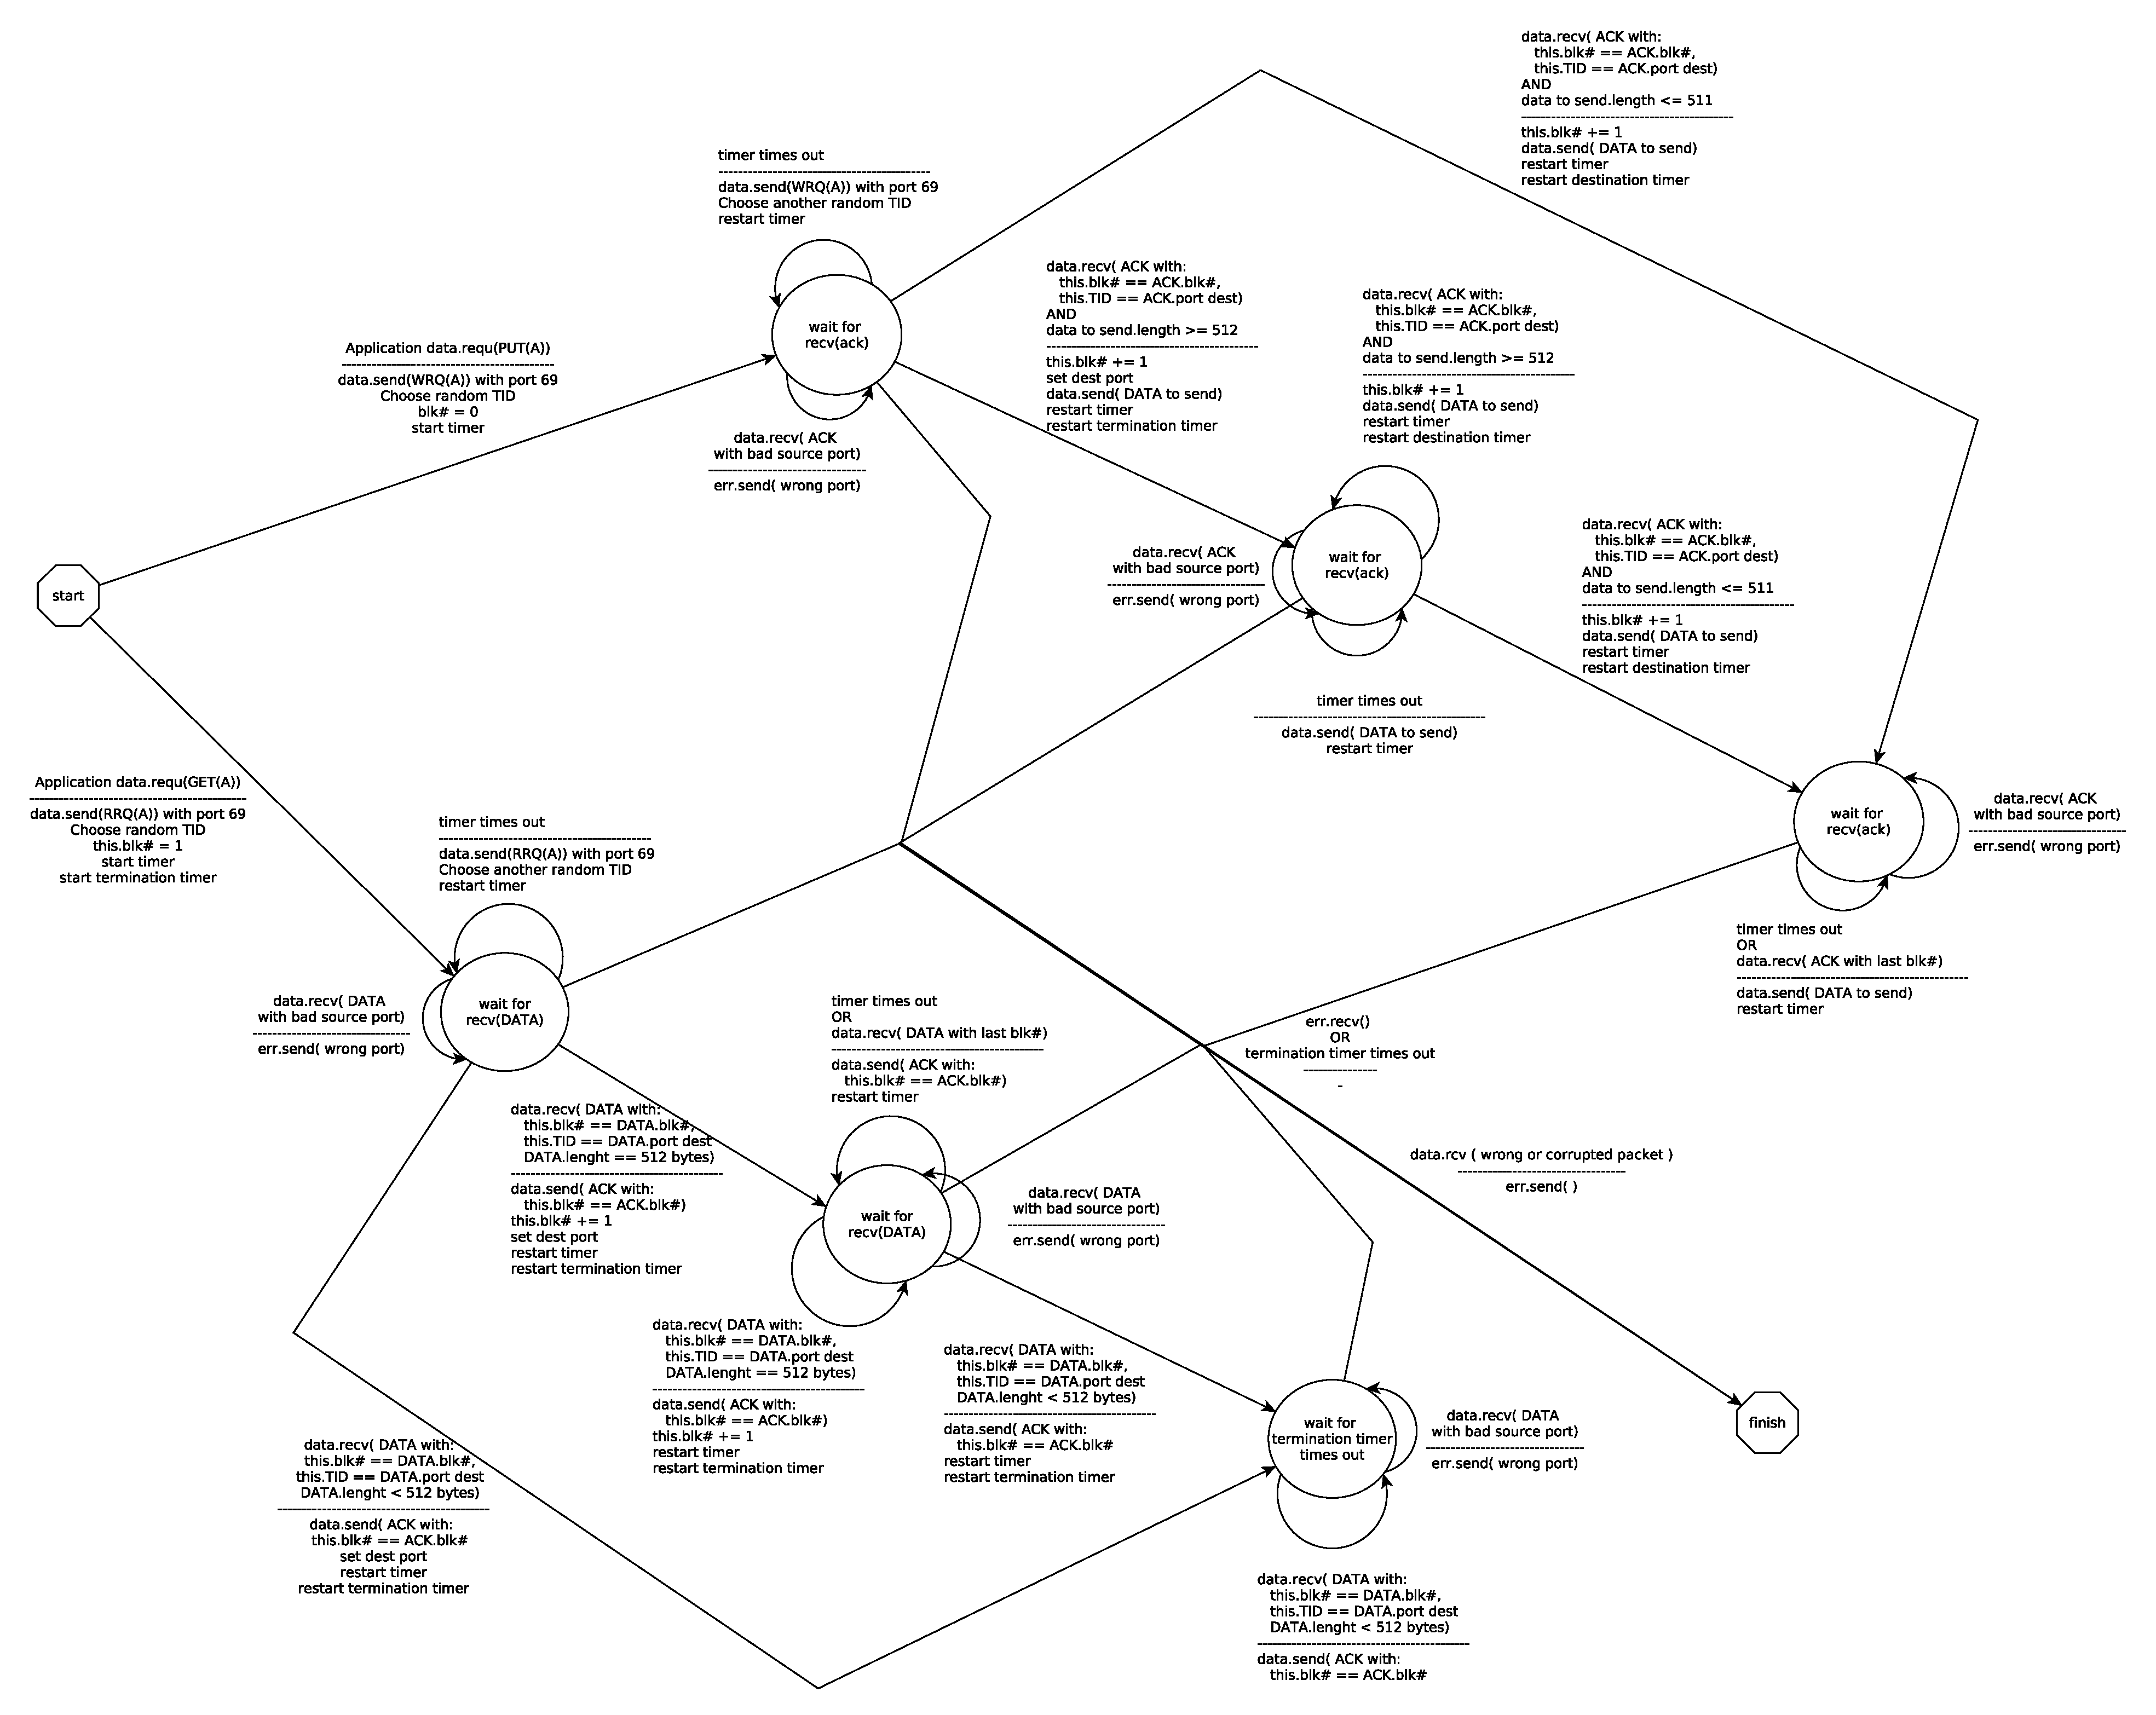
\includegraphics[width=1\textwidth]{ressources/client_state-machine.eps}
  \end{center}
  
  \subsubsection{Serveur}
  
  \begin{center}
	  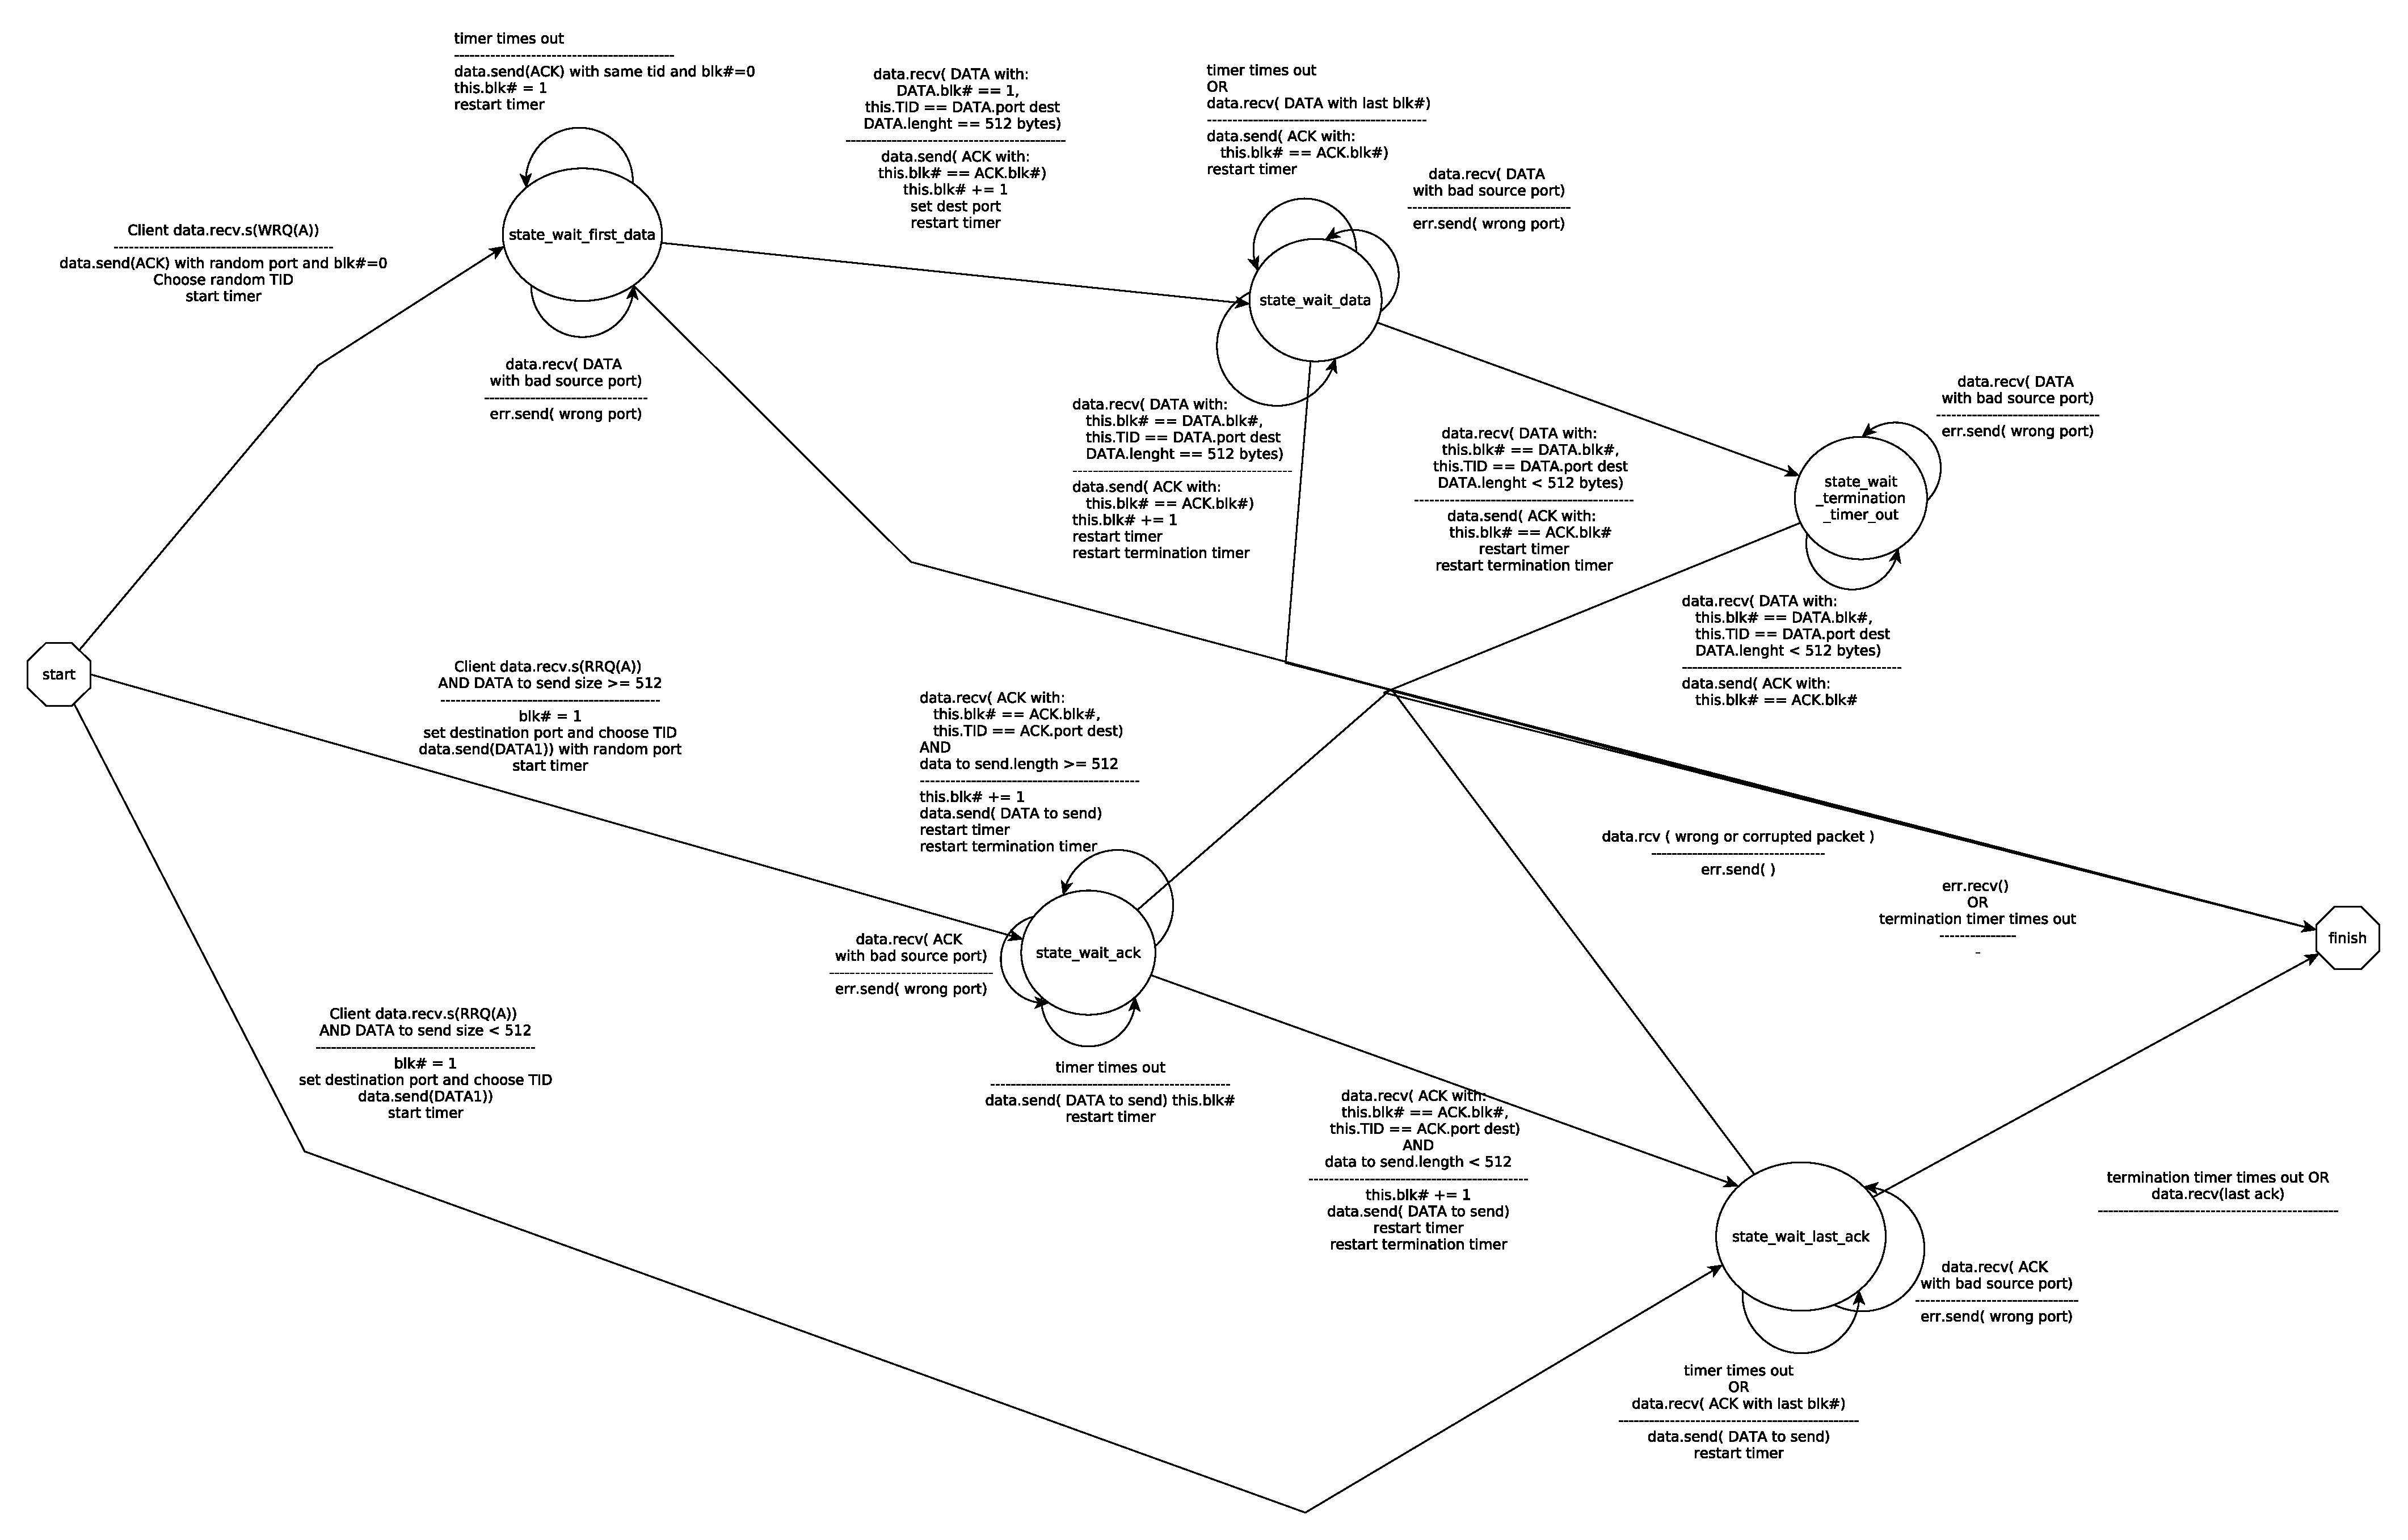
\includegraphics[width=1\textwidth]{ressources/server_state-machine.eps}
  \end{center}  
  
  \subsection{Cas d'erreur}
  
  \par Les cas d'erreurs suivants ont été analysés dans le but de tester la robustesse du protocole. Le premier exemple décrit la manière dont le protocole se comporte en cas de perte de paquets (coté client ou serveur). Les paquets sont simplement renvoyés en cas de timeout.
  
  \par Le deuxième cas (associé à ce qui est appelé syndrome de l’apprenti sorcier), décrit les erreurs qui peuvent survenir lors de délais dans la transmission des paquets.   Lorsque le délai est suffisamment grand, le paquet retardé est à nouveau envoyé, ce qui crée une duplication des paquets. Il faut s'assurer que cette duplication de paquets ne se propage pas pendant toute la durée du transfert. Ceci est résolu de la manière suivante: lorsqu'on reçoit un ACK concernant le paquet de données qu'on vient d'envoyer, on envoie le paquet de données suivant. Cependant, si on reçoit à nouveau le même ACK, on ne renvoie rien. 
  
  \par Le dernier cas illustré décrit le cas où un paquet de requête (RRQ ou WRQ) a été retardé. Suite au retard, un deuxième paquet de requête est envoyé, ce qui pourrait conduire à une double connexion entre le client et le serveur. Pour éviter ceci et d'envoyer deux fois le même fichier, lorsqu'un transfert de fichier débute, le client et le serveur choisissent un identifiant à utiliser tout le long du transfert. (identifiant inscrit comme ports UDP). Lorsque le client reçoit l'accord du serveur pour commencer le transfert de fichier, le client va enregistrer l'ID du serveur que celui-ci a envoyé pour le transfert de fichier. Lorsque le client reçoit le deuxième accord du serveur avec un ID différent, le client ne va pas initier une deuxième connexion avec le serveur car il est déjà avec une connexion avec celui-ci. Il n'y aura donc pas de double connexions. 
  
  \begin{center}
	  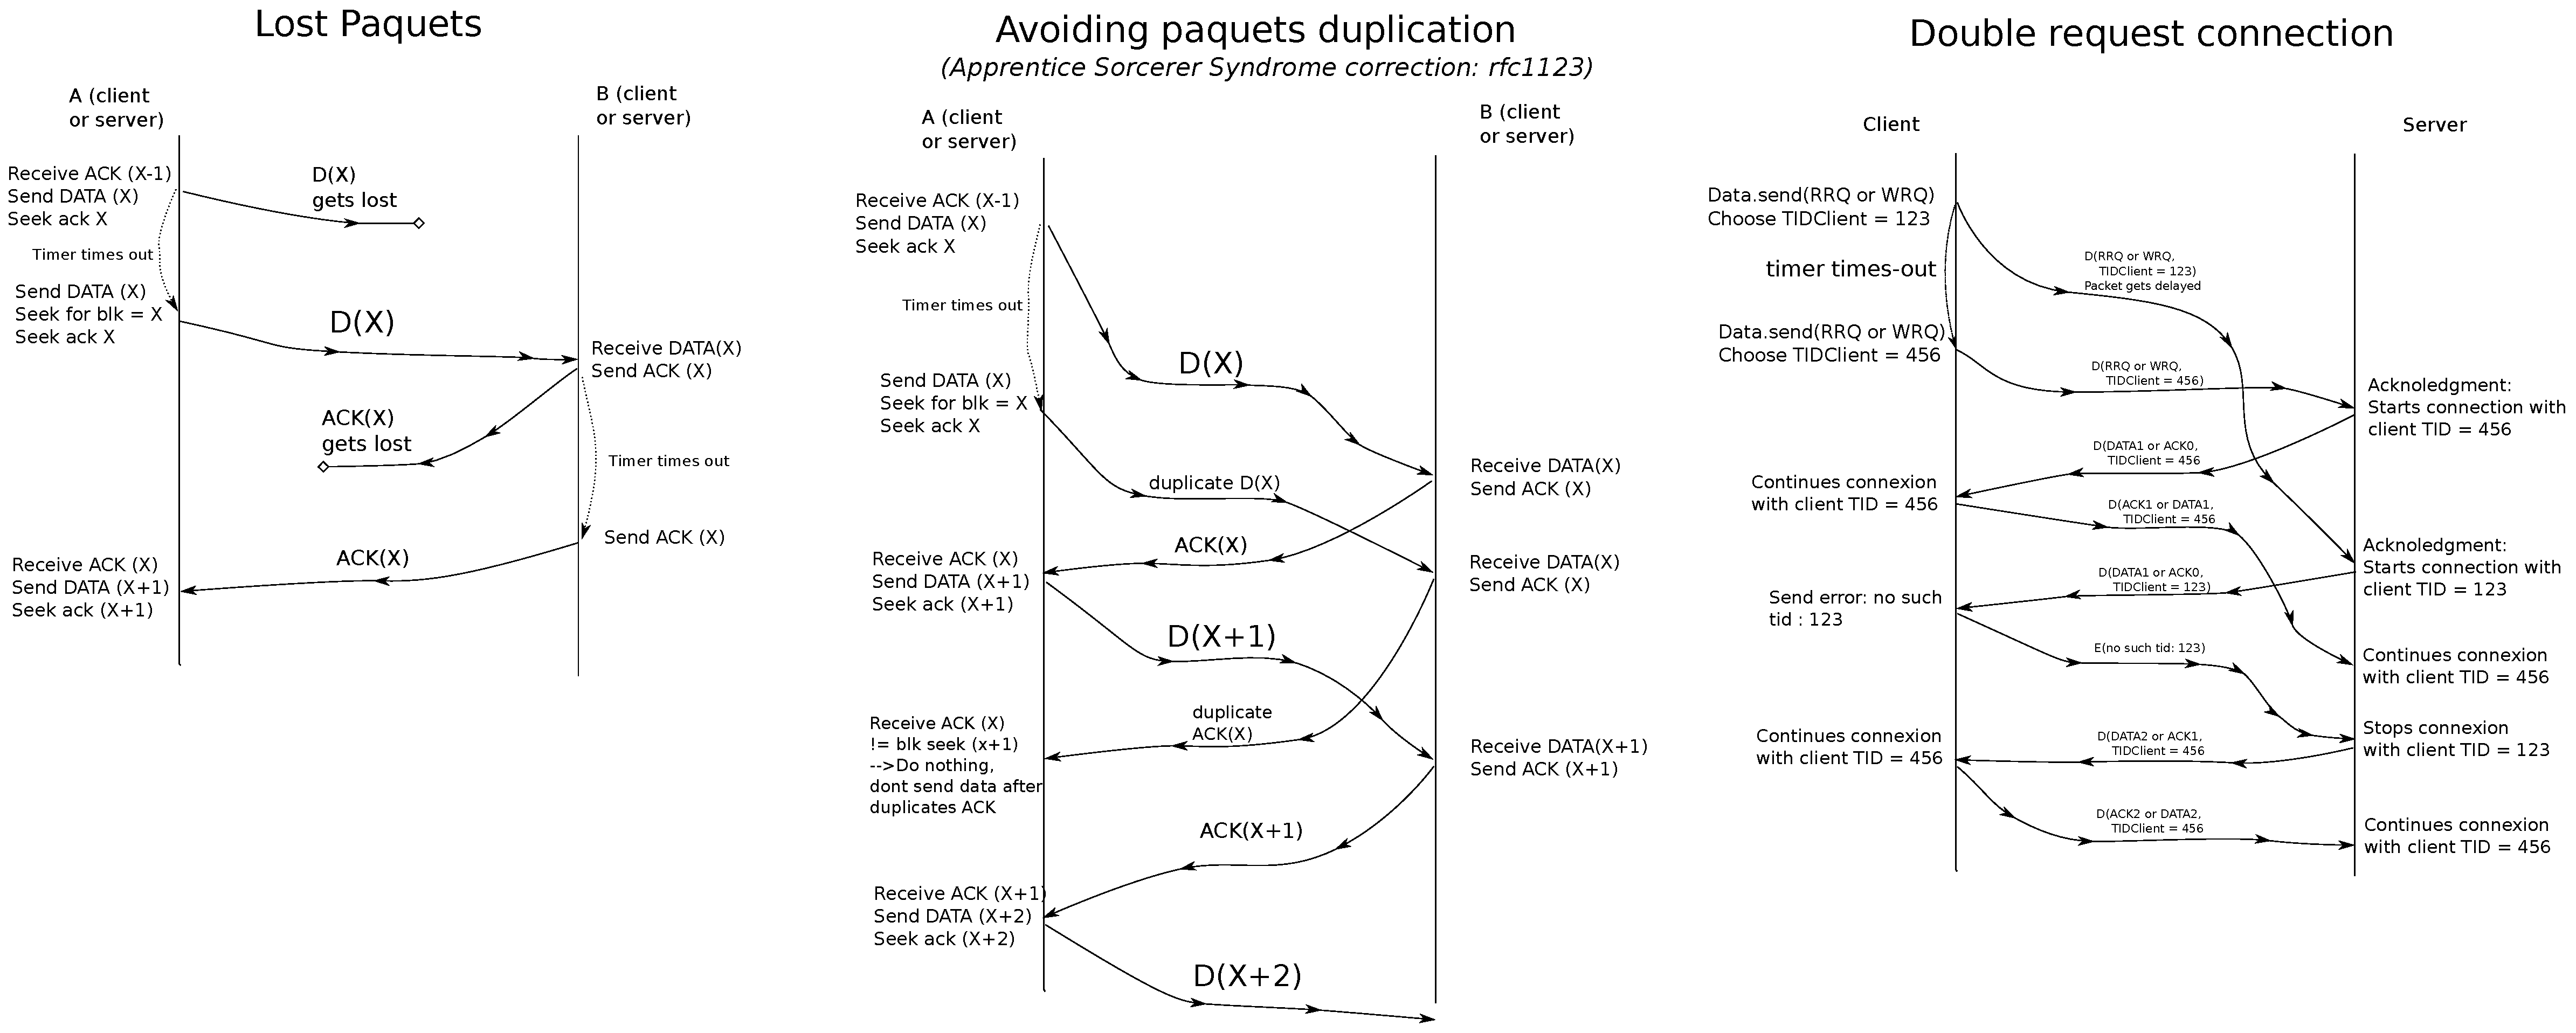
\includegraphics[width=1\textwidth]{ressources/errors_time-sequence.eps}  
  \end{center}	
	
  \section{Architecture du programme}
  
  \par L'architecture de notre implémentation a été définie comme suit. Deux fichiers client.py et server.py qui contiendront l'algorithme définit dans les machines d'états. 
  \\ Partant du principe que la manière de transférer les fichiers est la même pour le serveur et le client, nous avons définit un fichier utils.py qui contiendra les méthodes pour envoyer et recevoir des fichiers. Ces méthodes sont utilisées par le client et le serveur. 
  \\ Enfin, un fichier nommé packet.py, également utilisé par le serveur et le client, contient toutes les fonctions nécessaires pour encoder et décoder les paquets TFTP.
  
  \begin{center}
  	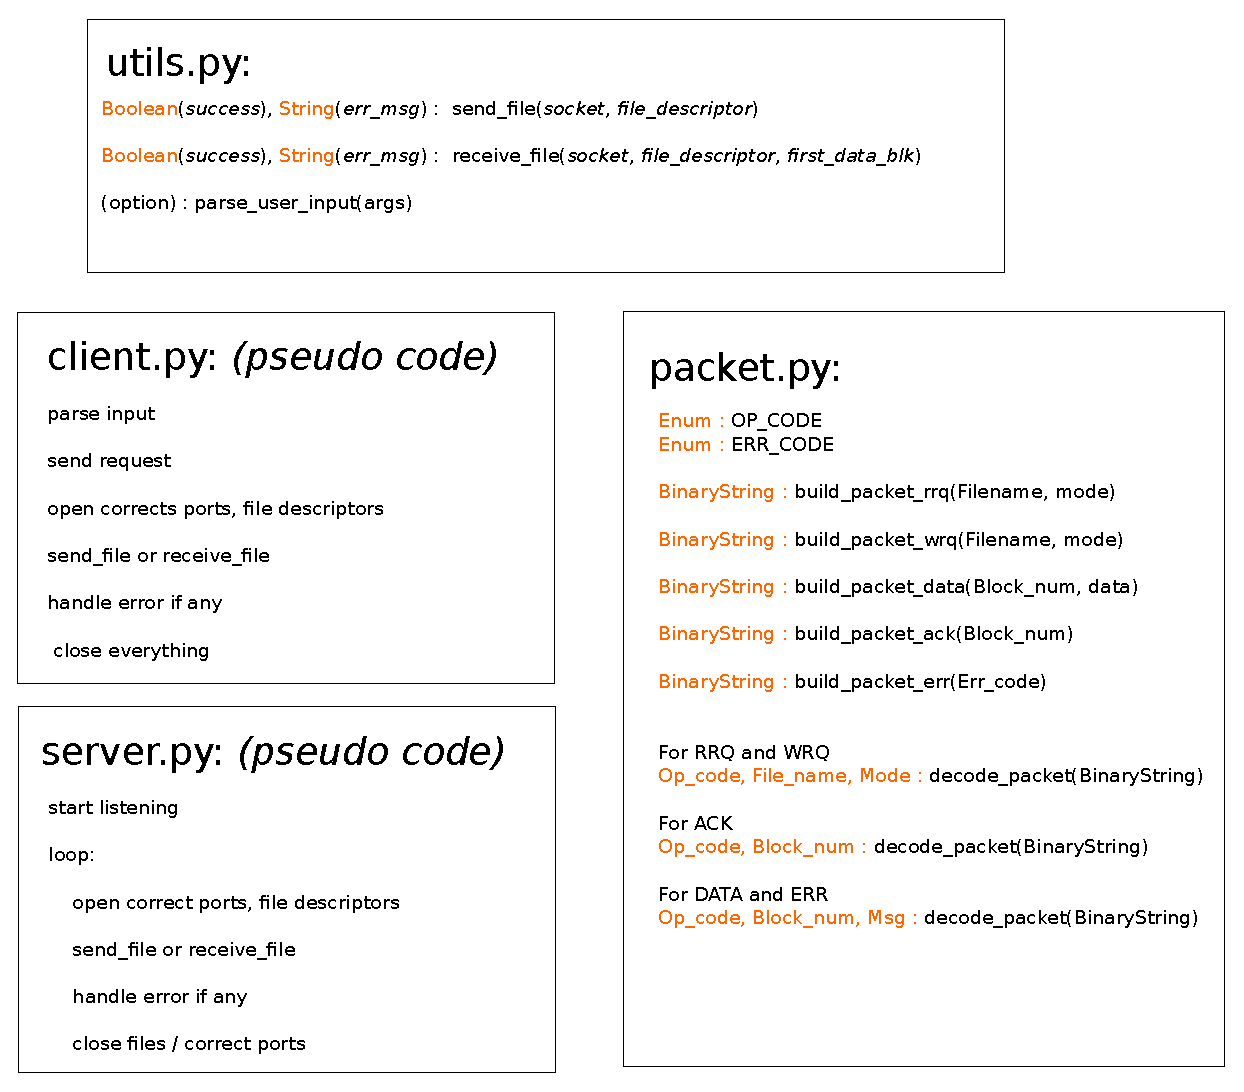
\includegraphics[width=1\textwidth]{ressources/architecture.eps}     
  \end{center}

\end{document}
